\section{ХОД РАБОТЫ}

\subsection{Текст задания}

Разработанная программа должна выводить список запущенных процессов в системе,
предварительно отсортировав его по приоритету, затем по времени запуска. Каждая строка
должна быть раскрашена в соответствии с приоритетом исполняемого процесса.

После списка запущенных процессов необходимо вывести статистическую информацию,
отражающую процентное соотношение процессов, имеющих конкретный приоритет
ко всем запущенным процессам.

Разработанная программа должна иметь возможность вывода справки по требованию пользователя.

\subsection{Детали реализации программы}

Получим список процессов, отсортируем его по приоритету, затем по времени создания процесса.
Команды, реализующие данные действия, представлены на рисунке~\ref{lst:get_and_sort_processes}.

\begin{lstlisting}[caption=Получение и сортировка списка запущенных процессов, label=lst:get_and_sort_processes]
  $processes = Get-WmiObject -Class win32_process
  $sorted_processes = $($processes | Sort-Object Priority, CreationDate)
\end{lstlisting}

Для вывода цветного текста в консоль PowerShell используем команду, представленную на рисунке~\ref{lst:color_text}.
\begin{lstlisting}[caption=Вывод цветного текста в консоль PowerShell, label=lst:color_text]
  $color = $_.Priority
  Write-Host $OutputString -ForegroundColor $color
\end{lstlisting}

Из рисунка~\ref{lst:color_text} видно, что цвет устанавливается в соответствии с приоритетом процесса.

\newpage
Процесс работы программы приведен на рисунке~\ref{fig:process}.

\begin{figure}[htbp]
  \centering
  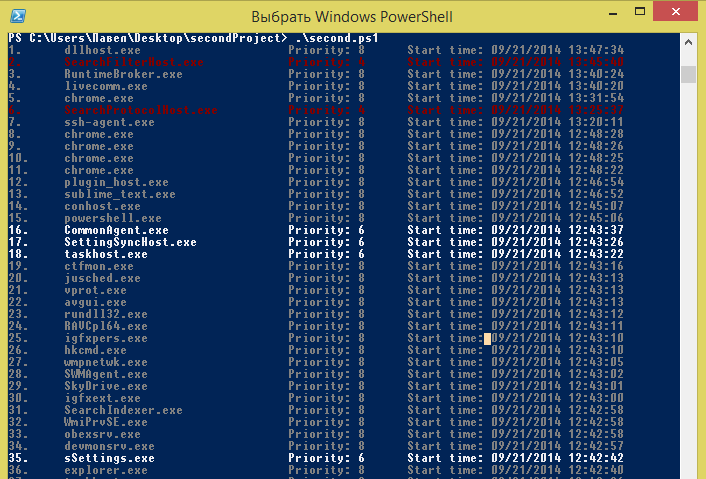
\includegraphics[width=150mm,height=90mm]{img/process}
  \caption{Вывод списка процессов с использованием командной оболочки PowerShell}\label{fig:process}
\end{figure}

Вывод статистической информации о процессах продемонстрирован на рисунке~\ref{fig:statistics}.

\begin{figure}[htbp]
  \centering
  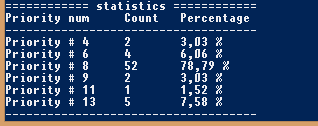
\includegraphics[width=80mm,height=35mm]{img/statistics}
  \caption{Вывод статистической информации о процессах \\ с помощью командной оболочки PowerShell}\label{fig:statistics}
\end{figure}

Исходный текст разработанной программы расположен в приложении~А.

\newpage
